\chapter{Funciones hiperbólicas}

\begin{tikzpicture}
	\fill [left color=red!50, right color=teal!50] (0,0) rectangle (6.5,.2);
	\fill [left color=teal!50, right color=blue!50] (6.5,0) rectangle (11.5,.2);
	\end{tikzpicture}

\vspace{5mm}
La funciones hipérbolicas son combinaciones de funciones exponenciales $e^x$ y $e^{-x}$ que aparecen con mucha frecuencia en aplicaciones físicas y pueden ser deducidas a partir de una hipérbola del mimo modo que las funciones circulares $\sin x,\, \cos x,\, ta x$ lo son de un círculo, de ahí su nombre. El primer científico que publicó un estudio de ellas fue Lambert (1728-1777), colega de Euler.

\vspace{1cm}
\section{Razones trigonométricas hiperbólicas}
\label{fhip}

\begin{tikzpicture}
	\fill [left color=red!50, right color=teal!50] (0,0) rectangle (3.5,.1);
	\fill [left color=teal!50, right color=blue!50] (3.5,0) rectangle (7.5,.1);
	\end{tikzpicture}
\vspace{0.5cm}


\begin{multicols}{2}
$\text{Área (OAP) } = \ \dfrac{\pi\, r^2}{2\pi}\,\phi= \dfrac \phi 2$

$\text{Área (OAB) } = \ \dfrac{1\cdot 1}{2}=\dfrac 1 2$

$$\dfrac{\text{Área sector (OAP) }}{\text{Área triángulo (OAB) }}=\dfrac{\phi/2}{1/2}=\ \phi$$

El arco $\phi$ se puede considerar como la razón  entre el área del sector $OAP$ y la del triángulo $OAB$
	\begin{figure}[H]
	\centering
	\includegraphics[width=.45\textwidth]{img-hiperbol/hiperbol01.png}
	\end{figure}
\end{multicols}
\begin{destacado}
	Podemos considerar el ángulo $\phi$ como el doble del área del sector circular $OAP$ en el círculo unidad.
\end{destacado}

\vspace{0.5cm}


\vspace{0.5cm}
\begin{multicols}{2}
$\quad$

Consideremos ahora la hipérbola $\ x^2-y^2=1$.

\begin{destacado}
Análogamente, podemos considerar el ángulo $\theta$ como el doble del área del sector $OAP$ en la hipérbola unidad.
\end{destacado}

\emph{$\theta$ es la medida hiperbólica del ángulo $AOP$}.

	\begin{figure}[H]
	\centering
	\includegraphics[width=.45\textwidth]{img-hiperbol/hiperbol02.png}
	\end{figure}
\end{multicols}


$\theta=\dfrac{ \text{Área sector (OAP)} }{ \text{Área triángulo (OAB)} }=\dfrac{\text{Área sector (OAP) }}{ 1/2 }$

$\text{Área sector (OAP)}=\text{Área triángulo (OCP)}-\text{Área  (ACP)}=\dfrac 1 2 x\, y - \text{Área  (ACP)}$

$\text{Área  (ACP)}=\displaystyle \int_1^x \sqrt{z^2-1}\, \dd z= \textcolor{gris}{\mqty(\text{ver al final} \\ \text{del la capítulo})}=\dfrac x 2 \sqrt{x^2-1}-\dfrac 1 2 \, \ln \, |x+\sqrt {x^2-1}|$

Luego, $\text{Área sector (OAP)}=\dfrac{xy}2-\dfrac x 2 \sqrt{x^2-1}+\dfrac 1 2 \, \ln |x+\sqrt {x^2-1}|$

Como estamos en la hipérbola, $\ \sqrt{x^2-1}=y$, con lo que

$\text{Área  (ACP)}=\cancel{\dfrac{xy}{2}}-\cancel{\dfrac{xy}{2}}+\dfrac 1 2 \ln  |x+y|=\dfrac 1 2 \ln |x+y|$

Como el área del triángulo $AOB$ es $\dfrac 1 2$, finalmente obtenemos:

$$\theta = \dfrac {\dfrac 1 2 \ln |x+y|}{\dfrac 1 2 } \quad \rightarrow \qquad \boxed{ \ \subrayado{\ \boldsymbol{\theta \ = \ \ln\, |x+y|} \ } \ } $$

\begin{cuadro-naranja}
Como en las funciones circulares (seno, coseno y tangente) se definen las funciones hiperbólicas (seno hiperbólico, cosen hiperbólico y tangente hiperbólica):

$$\sinh \theta = y= \overline{PC};\qquad \cosh \theta=x=\overline{OC};\qquad \tanh \theta=\dfrac{\sinh \theta}{\cosh \theta}=\dfrac y x$$	
\end{cuadro-naranja}

Como exponencial y logarítmica son funciones inversas una de la otra, $\ e^{\ln x}=x$, por lo que:

$e^\theta = e^{\ln\, |x+y|}= x+y \qquad e^{-\theta}=\dfrac 1{e^\theta}= \dfrac 1{x+y}$

Con un poco de álgebra y la ecuación de la hipérbola $(\textcolor{red}{x^2-y^2=1})$ podremos expresar el seno hiperbólico $(y)$ y el coseno hiperbólico $(x)$ en función de $\theta$.

$\boldsymbol{\sinh \theta}=y=y\dfrac 2 2 = \dfrac{2y}2 \dfrac{x+y}{x+y}=\dfrac{2xy+2y^2}{2(x+y)}=\dfrac{y^2+2xy+y^2}{2(x+y)}=\dfrac{\textcolor{red}{x^2-1}+2xy+y^2}{2(x+y)}=\dfrac{x^2+2xy+y^2-1}{2(x+y)}=\dfrac{(x+y)^2-1}{2(x+y)}=\dfrac{\dfrac{(x+y)^2-1}{x+y}}{2}=\dfrac{x+1-\dfrac {1}{x+y}}{2}=\boldsymbol{\dfrac{e^\theta-e^{-\theta}}{2}}$

\vspace{3mm}
$\boldsymbol{\cosh \theta}=x=x\dfrac 2 2 = \dfrac{2x}2 \dfrac{x+y}{x+y}=\dfrac{2x^2+2xy}{2(x+y)}=\dfrac{x^2+2xy+x^2}{2(x+y)}=\dfrac{\textcolor{red}{y^2+1}+2xy+x^2}{2(x+y)}=\dfrac{x^2+2xy+y^2+1}{2(x+y)}=\dfrac{(x+y)^2+1}{2(x+y)}=\dfrac{\dfrac{(x+y)^2+1}{x+y}}{2}=\dfrac{x+1+\dfrac {1}{x+y}}{2}=\boldsymbol{\dfrac{e^\theta+e^{-\theta}}{2}}$

\vspace{2mm}
A partir de esta dos relaciones se definen las demás: $\ \tanh \theta, \, \coth \theta, \, \sech \theta,\, \csch\, \theta$. 

\vspace{10mm}


\begin{definition}

\begin{table}[H]
\centering
\begin{tabular}{lll}
$\boldsymbol{\sinh \theta=\dfrac{e^\theta-e^{-\theta}}{2}}$  & $\qquad \qquad$ & $\boldsymbol{\cosh \theta=\dfrac{e^\theta+e^{-\theta}}{2}}$ \\ \\
$\tanh \theta=\dfrac{\sinh \theta}{\cosh \theta}=\dfrac{e^\theta-e^{-\theta}}{e^\theta+e^{-\theta}}$ & & $\coth \theta=\dfrac{\cosh \theta}{\sinh \theta}=\dfrac{e^\theta+e^{-\theta}}{e^\theta-e^{-\theta}}$ \\ \\
$\sech \theta = \dfrac{1}{\cosh \theta}=\dfrac{2}{e^\theta+e^{-\theta}}$  &  & $\csch \theta = \dfrac{1}{\sinh \theta}=\dfrac{2}{e^\theta-e^{-\theta}}$
\end{tabular}
\end{table}
\end{definition}






\vspace{1cm}
\section{Identidades trigonométricas hiperbólicas}

\begin{tikzpicture}
	\fill [left color=red!50, right color=teal!50] (0,0) rectangle (3.5,.1);
	\fill [left color=teal!50, right color=blue!50] (3.5,0) rectangle (7.5,.1);
	\end{tikzpicture}
\vspace{0.5cm}

\begin{theorem}

\begin{equation}
\label{EFTH}	
\large{ \boxed{ \ \boldsymbol{ \cosh^2 x-\sinh^2 x=1 } \ } }	
\end{equation}
\end{theorem}

\normalsize{\underline{Demostración}:} 

$\left( \dfrac{e^x+e^{-x}}{2} \right)^2-\left( \dfrac{e^x-e^{-x}}{2} \right)^2=\dfrac{e^{2x}+2+e^{-2x}-e^{2x}+2-e^{-2x}}{4}=\dfrac 4 4 = 1 \qquad \qquad \Box$

\vspace{5mm}
\begin{theorem}

\begin{equation}
\label{EFTH2}
\large{ \boxed{ \ \boldsymbol{ \tanh^2 x+\sech^2 x=1 } \ } }	
\end{equation}
\end{theorem}

\normalsize{\underline{Demostración}:} 

$\left(\dfrac{\sinh x}{\cosh x} \right)^2-\left( \dfrac{1}{\cosh x}\right)^2=\dfrac{\sinh^2 x+1}{\cosh^2 x}= \text{(th. \ref{EFTH} )} = \dfrac 1 1 =1 \qquad \qquad \Box$


\vspace{5mm}
\begin{theorem}

$$\large{ \boxed{ \ \boldsymbol{ \coth^2 x-\csch^2 x=1 } \ } }	$$
\end{theorem}

\normalsize{\underline{Demostración}:} 

$\left(\dfrac{\cosh x}{\sinh x} \right)^2-\left( \dfrac{1}{\sinh x}\right)^2=\dfrac{\cosh^2 x-1}{\sinh^2 x}= \text{(th. \ref{EFTH} )} = \dfrac 1 1 =1 \qquad \qquad \Box$


\vspace{5mm}
\begin{theorem}

$$\large{ \boxed{ \ \boldsymbol{ \sinh 2x=2\, \sinh x \, \cosh x } \ } }	$$
\end{theorem}

\normalsize{\underline{Demostración}:} 

$2\sinh x \, \cosh x=2 \dfrac{e^x-e^{-x}}{2} \dfrac{e^x+e^{-x}}{2} =\dfrac{e^{2x}-e^{-2x}}{2} =\sinh 2x\qquad \qquad \Box$

\vspace{5mm}
\begin{theorem}

$$\large{ \boxed{ \ \boldsymbol{ \cosh 2x= \cosh^2 x + \sinh^2 x } \ } }	$$
\end{theorem}

\normalsize{\underline{Demostración}:} 

$\cosh^2 x+\sinh^2 x=\left( \dfrac{e^x+e^{-x}}{2} \right)^2 +\left( \dfrac{e^x-e^{-x}}{2} \right)^2 = \dfrac{e^{2x}+1+e^{-2x}+e^{2x}-1+e^{-2x}}{4}=  \dfrac{e^{2x}+e^{-2x}}{2} =\cosh 2x\qquad \qquad \Box$

\vspace{5mm}
\begin{theorem}

\begin{table}[H]
\centering
\begin{tabular}{ll}
$\sinh(x+y)=\sinh x \cosh y+ \cosh x\sinh y$ ;      & $\sinh(x-y)=\sinh x \cosh y- \cosh x\sinh y$   \\ \\
$\cosh (x+y)=\cosh x \cosh y + \sinh x \sinh y$ ;    & $\cosh (x-y)=\cosh x \cosh y - \sinh x \sinh y$
\end{tabular}
\end{table}
\end{theorem}

\normalsize{\underline{Demostración}:} \emph{se deja como ejercicio}.


\vspace{5mm}
\begin{theorem}

\begin{table}[H]
\centering
\begin{tabular}{ll}
$ \sinh x + \sinh y = 2 \sinh \dfrac{x+y}2 \cosh \dfrac{x-y}2$   &   $ \sinh x - \sinh y = 2 \cosh \dfrac{x+y}2 \sinh \dfrac{x-y}2$ \\ \\
$ \cosh x + \cosh y = 2 \cosh \dfrac{x+y}2 \cosh \dfrac{x-y}2$    & $ \cosh x + \cosh y = 2 \sinh \dfrac{x+y}2 \sinh \dfrac{x-y}2$
\end{tabular}
\end{table}
\end{theorem}

\normalsize{\underline{Demostración}:} \emph{se deja como ejercicio}.


\vspace{1cm}
\section{Funciones hiperbólicas}

\begin{tikzpicture}
	\fill [left color=red!50, right color=teal!50] (0,0) rectangle (3.5,.1);
	\fill [left color=teal!50, right color=blue!50] (3.5,0) rectangle (7.5,.1);
	\end{tikzpicture}
\vspace{0.5cm}

	
\begin{figure}[H]
	\centering
	\includegraphics[width=1\textwidth]{img-hiperbol/hiperbol05.png}
	\end{figure}


\begin{figure}[H]
	\centering
	\includegraphics[width=.6\textwidth]{img-hiperbol/hiperbol04.png}
	\end{figure}


\vspace{1cm}
\section{Funciones hiperbólicas inversas} 

\begin{tikzpicture}
	\fill [left color=red!50, right color=teal!50] (0,0) rectangle (3.5,.1);
	\fill [left color=teal!50, right color=blue!50] (3.5,0) rectangle (7.5,.1);
	\end{tikzpicture}
\vspace{0.5cm}

Las funciones inversas de seno hiperbólico, coseno hiperbólico y tangente hiperbólica reciben, respectivamente, los nombres de \emph{argumento seno hiperbólico}, \emph{argumento coseno hiperbólico} y \emph{argumento tangente hiperbólico}: $\ \mathrm{arg\, sinh} x,\, \mathrm{arg\, cosh} x \text{ y } \mathrm{arg\, tanh} x$.

\textcolor{gris}{Una función y su inversa ($x \leftrightarrow y$) son simétricas respecto de la bisectriz del primer y tercer cuadrante ($y=x$). Como el coseno hiperbólico no es inyectivo, su inversa no es una función, solo una correspondencia. Para arreglar esto, nos quedamos con la zona de inyectividad del coseno hiperbólico, $[0,+\infty[$.}


\begin{figure}[H]
	\centering
	\includegraphics[width=1\textwidth]{img-hiperbol/hiperbol06.png}
	\end{figure}


\begin{figure}[H]
	\centering
	\includegraphics[width=.5\textwidth]{img-hiperbol/hiperbol07.png}
	\end{figure}

Así como las funciones hiperbólicas son combinaciones de funciones exponenciales, sus inversas deberías tener que ver con los logaritmos:

\vspace{5mm}$\triangleright \quad$ \textbf{Argumento seno hiperbólico}.

$y=\mathrm{arg\, sinh} x \ \leftrightarrow x=\sinh y=\dfrac{e^y-e^{-y}}{2}$

$2x=e^y-e^{-y}\, , \  $ multiplicando por $e^y\, : \ \ 2xe^y=e^{2y}-1 \ \to \ (e^y)^2-2xe^y-1=0$ 

Ecuación de $2^o$ grado en $e^y \ \Rightarrow \ e^y=\dfrac{4x\pm \sqrt{4x^2+4}}{2\cdot 1}=x\pm \sqrt{x^2+1}$

Tomando logaritmos: $\quad y = \ \boxed{ \ \boldsymbol{\mathrm{arg\, sinh} x\ = \ \ln \left( x+\sqrt{x^2+1} \right) } \ } \ , \quad x\in ]-\infty,+\infty[$

Hemos tomado el signo $\, + \, $ porque el $\, - \, $ da un argumento negativo para el logaritmo.

\vspace{5mm}$\triangleright \quad$ \textbf{Argumento coseno hiperbólico}.

$y=\mathrm{arg\, cosh} x \ \leftrightarrow x=\cosh y=\dfrac{e^y+e^{-y}}{2}$

$2x=e^y+e^{-y}\, , \  $ multiplicando por $e^y\, : \ \ 2xe^y=e^{2y}+1 \ \to \ (e^y)^2-2xe^y+1=0$ 

Ecuación de $2^o$ grado en $e^y \ \Rightarrow \ e^y=\dfrac{4x\pm \sqrt{4x^2-4}}{2\cdot 1}=x\pm \sqrt{x^2-1}$

Tomando logaritmos: $\quad y = \ \boxed{ \ \boldsymbol{\mathrm{arg\, cosh} x\ = \ \ln \left( x+\sqrt{x^2-1} \right) } \ } \ , \quad x\in ]1,+\infty[$

Hemos tomado el signo $\, + \, $ porque el $\, - \, $ da un argumento negativo para el logaritmo.

\vspace{5mm}$\triangleright \quad$ \textbf{Argumento tangente hiperbólica}.

$y=\mathrm{arg\, tanh} x \ \leftrightarrow x=\tanh y=\dfrac{e^y-e^{-y}}{e^y+e^{-y}}=\dfrac{e^{2y}-1}{e^{2y}+1}$

Despejando $\ \ x(e^{2y}+1)=e^{2y}-1 \ \to \ xe^{2y}-e^{2y}=-x-1 \ \to \ e^{2y}=\dfrac{1+x}{1-x}$ 

Tomando logaritmos: $\quad y = \ \boxed{ \ \boldsymbol{\mathrm{arg\, tanh} x }\ = \ \dfrac 1 2 \ln \dfrac {1+x}{1-x} =\ \boldsymbol{ \ln \sqrt{\dfrac {1+x}{1-x}  } } \ } \ , \quad x\in ]-1,+1[$

Hemos tomado el signo $\, + \, $ porque el $\, - \, $ da un argumento negativo para el logaritmo.


\vspace{1cm}
\section{Derivadas de funciones hiperbólicas}

\begin{tikzpicture}
	\fill [left color=red!50, right color=teal!50] (0,0) rectangle (3.5,.1);
	\fill [left color=teal!50, right color=blue!50] (3.5,0) rectangle (7.5,.1);
	\end{tikzpicture}
\vspace{0.5cm}

$\triangleright \quad \boldsymbol{y=\sinh x} =\dfrac{e^x-e^{-x}}{2} \ \to$

$\to \ \displaystyle \boxed{ \subrayado{ \  \ \boldsymbol{ \dv{x}  \, \sinh x} \ } \ } \ =y'= \dfrac{ e^x-e^{-x} (-1) } { 2 } =\dfrac{e^x+e^{-x}}{2} = \ \boxed{ \ \subrayado{ \  \boldsymbol{\cosh x} \ } \ }$

\vspace{0.5cm}

$\triangleright \quad \boldsymbol{y=\cosh x} =\dfrac{e^x+e^{-x}}{2} \ \to$

$\to \ \displaystyle \boxed{ \subrayado{ \  \ \boldsymbol{ \dv{x}  \, \cosh x} \ } \ } \ =y'= \dfrac{ e^x+e^{-x} (-1) } { 2 } =\dfrac{e^x-e^{-x}}{2} = \ \boxed{ \ \subrayado{ \  \boldsymbol{\sinh x} \ } \ }$

\vspace{0.5cm}

$\triangleright \quad \boldsymbol{y=\tanh x} =\dfrac{\sinh x}{\cosh x} \ \to$

$\to \ \displaystyle \boxed{ \subrayado{ \  \ \boldsymbol{ \dv{x}  \, \tanh x} \ } \ } \ =y'= \dfrac{ \cosh^2 x-\sinh^2 x } { \cosh^2 x } =\dfrac{1}{\cosh^2 x} = \ \boxed{ \ \subrayado{ \  \boldsymbol{\sech^2 x} \ } \ }$

\vspace{1cm}

Del mismo modo:

\vspace{-0.5cm}

$$\displaystyle \dv{x} \, \coth x =-\csch^2 x;\qquad \dv{x} \, \sech x =-\sech x \, \tanh x;\qquad \dv{x} \, \csch x=-\csch x\, \coth	x$$

La demostración de estas tres últimas derivadas se deja como ejercicio.

\vspace{1.5cm}

$\triangleright \quad \boldsymbol{y=\mathrm{arg\, sinh} x} =\ln(x+\sqrt{x^2+1}) \ \to$

$\to \ \displaystyle \boxed{ \subrayado{ \  \ \boldsymbol{ \dv{x}  \, \mathrm{arg\, sinh} x } \ } \ } \ =y'= \dfrac{1+\dfrac{\cancel{2} x}{\cancel{2} \sqrt{x^2+1}}}{x+\sqrt{x^2+1}} = \dfrac{x+\sqrt{x^2+1}}{\sqrt{x^2+1} (x+\sqrt{x^2+1})}  = \ \boxed{ \ \subrayado{ \  \boldsymbol{ 
\dfrac 1 {\sqrt {x^2+1}} } \ } \ }$


\vspace{0.5cm}

$\triangleright \quad \boldsymbol{y=\mathrm{arg\, cosh} x} =\ln(x+\sqrt{x^2-1}) \ \to$

$\to \ \displaystyle \boxed{ \subrayado{ \  \ \boldsymbol{ \dv{x}  \, \mathrm{arg\, cosh} x } \ } \ } \ =y'= \dfrac{1+\dfrac{\cancel{2} x}{\cancel{2} \sqrt{x^2-1}}}{x+\sqrt{x^2-1}} = \dfrac{x+\sqrt{x^2-1}}{\sqrt{x^2+1} (x+\sqrt{x^2+1})}  = \ \boxed{ \ \subrayado{ \  \boldsymbol{ \dfrac 1 {\sqrt{x^2-1} } } \ } \ }$

\vspace{0.5cm}

$\triangleright \quad \boldsymbol{y=\mathrm{arg\, tanh} x} =\ln \sqrt{\dfrac{1+x}{1-x}} \ \to$

$\to \ \displaystyle \boxed{ \subrayado{ \  \ \boldsymbol{ \dv{x}  \, \mathrm{arg\, tanh} x } \ } \ } \ =y'= \dfrac {1} {\cancel{2}} \dfrac 1{\dfrac{1+x}{\bcancel{1-x}}} \dfrac{\cancel{1(1-x)-(1+x)(-1)}}{(1-x)^{\bcancel{2}}} = \ \boxed{ \ \subrayado{ \  \boldsymbol{ \dfrac 1 {1-x^2}   } \ } \ }$



\vspace{1cm}
\section{Integrales de funciones hiperbólicas}

\begin{tikzpicture}
	\fill [left color=red!50, right color=teal!50] (0,0) rectangle (3.5,.1);
	\fill [left color=teal!50, right color=blue!50] (3.5,0) rectangle (7.5,.1);
	\end{tikzpicture}
\vspace{0.5cm}

\begin{table}[H]
\centering
\begin{tabular}{lll}
$\displaystyle \int \sinh u\, \dd u=\cosh u + \mathcal C$ & $\quad \displaystyle \int \cosh u\, \dd u=\sinh u + \mathcal C \quad $ & $\displaystyle \int \tanh u\, \dd u=\ln(\cosh u)+ \mathcal C$
\end{tabular}
\end{table}

\begin{table}[H]
\centering
\begin{tabular}{lll}
$\displaystyle \int \sech^2 u\, \dd u= \tanh u + \mathcal C$ & $\qquad$  & $\displaystyle \int \csch^2 u\, \dd u= \coth u + \mathcal C$
\end{tabular}
\end{table}

\begin{table}[H]
\centering
\begin{tabular}{lll}
$\displaystyle \int \dfrac{\dd u}{\sqrt{a^2+u^2}}=\mathrm{arg\, senh} \dfrac u a + \mathcal C$ & $\displaystyle \int \dfrac{\dd u}{\sqrt{u^2-a^2}}=\mathrm{arg\, cosh} \dfrac u a + \mathcal C$  & $\displaystyle \int \dfrac{\dd u}{a^2-u^2}= \dfrac 1 a \mathrm{arg\, tanh} \dfrac u a + \mathcal C$
\end{tabular}
\end{table}


\vspace{1cm}
\section{Aplicaciones de funciones hiperbólicas}

\begin{tikzpicture}
	\fill [left color=red!50, right color=teal!50] (0,0) rectangle (3.5,.1);
	\fill [left color=teal!50, right color=blue!50] (3.5,0) rectangle (7.5,.1);
	\end{tikzpicture}
\vspace{0.5cm}

\begin{miejercicio}
	
	El Arco Gateway, o la Puerta hacia el Oeste, es la parte más importante del Monumento a la Expansión Nacional de Jefferson en San Luis, Misuri (USA). Se construyó como un monumento conmemorativo de la expansión hacia el oeste de los Estados Unidos. Es el monumento más alto hecho por el hombre en los Estados Unidos y tiene forma de arco catenario aplastado. En el centro tiene 192 m de altura y la bases mide 192.28 m.
	
	\vspace{2mm}La forma catenaria del arco satisface, aproximadamente, la ecuación $\ y=231-30\cosh \left( \dfrac x {39} \right)$.
	Determínese la longitud total del arco y el área encerrada por éste.
\end{miejercicio}


\vspace{3mm}
\begin{multicols}{2}
\begin{figure}[H]
	\centering
	\includegraphics[width=.4\textwidth]{img-hiperbol/hiperbol08.png}
	\end{figure}
\begin{figure}[H]
	\centering
	\includegraphics[width=.5\textwidth]{img-hiperbol/hiperbol09.png}
	\end{figure}	
\end{multicols}

$L=2\displaystyle \int_0^{96.14} \sqrt{1+\left( \dv{y}{x} \right)} \, \dd x= 2\int_0^{96.14} \sqrt{ 1+ \left( - \sinh \left( \dfrac{x}{39} \right) \right)^2 } =2 \int_0^{96.14} \cosh  \left( \dfrac{x}{39} \right) =$

$= \displaystyle 2\,  \left[ 39 \sinh  \left( \dfrac{x}{39} \right) \right]_0^{96.14}=\boldsymbol{ 455.52 \, \mathrm{m} } $ 

\vspace{3mm}

$A=\displaystyle 2 \int_0^{96.14} \left[ 231-39 \cosh \left( \dfrac{x}{39} \right) \right] \, \dd x = 2 \, \left[ 231 x- (39)^2 \, \sinh \left( \dfrac{x}{39} \right) \right]_0^{96.14}= \boldsymbol{26651.42\, \mathrm{m}^2}$

\vspace{10mm}

\begin{miejercicio}

El Radón es un gas que puede difundirse a través de materiales sólidos como tabiques y cemento. Sí la dirección de la difusión en un muro de cimentación es perpendicular a la superficie entonces la concentración de Radón $f(x)$ (en $\mathrm{J\, cm}^3$) en los poros llenos de aire existentes en el muro, a una distancia $x$ de la superficie exterior puede ser aproximada por la expresión: $\ f(x) = A \sinh (\rho x)+ B \ cosh (\rho x)+ K\, , $ donde la constante $\rho$ depende de la porosidad del muro, de la vida medía del Radón y de un coeficiente de difusión; la constante $K$ es la máxima concentración de Radón en los poros llenos de aire; y $A$ y $B$ son constantes que dependen de las condiciones iniciales. Mostrar que $y=f(x)$ es solución de la ecuación de difusión:	 $\ \displaystyle \dv[2]{y}{x}-\rho^2 y+ \rho^2 k=0$
\end{miejercicio}

\vspace{5mm}

$y= A \sinh (\rho x)+ B \ cosh (\rho x)+ K \quad \to \quad \displaystyle \dv{y}{x}=A\rho \cosh (\rho x)+B\rho \sinh (\rho x) \quad \to \quad $

$\displaystyle \dv[2]{y}{x}=A\rho^2 \sinh (\rho x)+B\rho^2 \cosh (\rho x)$

Sustituyendo: $\quad A\rho^2 \sinh (\rho x)+B\rho^2 \cosh (\rho x)-\rho^2 \left[  A \sinh (\rho x)+ B \ cosh (\rho x)+ K  \right] +\rho^2 k =0$




%%%%%%%%%%%%%%%%. FINAL del capítulo.
\vspace{10mm}
\newpage %%%%%%%%%%%%%%%%%%%%%%%%%%%%%%%
\color{gris}
\rule{250pt}{0.1pt}

Demostración de la integral de la sección \ref{fhip}:

Veamos que $\quad \displaystyle I=\int_1^x \sqrt{z^2-1}\, \dd z\ = \ \dfrac x 2 \sqrt{x^2-1}-\dfrac 1 2 \, \ln \, |x+\sqrt {x^2-1}|$

Sustitución trigonimétrica: $\ z=\sec w$

\begin{multicols}{2}
$z=\sec w=\dfrac 1{\cos w} \leftrightarrow \cos w=\dfrac 1 z$

$\sin w=\dfrac{\sqrt{z^2-1}}{z};\ \ \tan z=\sqrt{z^2-1}$

$\mathrm{d}z=\sec w\, \tan w\, \mathrm{d}w$

$\sqrt{z^2-1}=\tan w$
\begin{figure}[H]
	\centering
	\includegraphics[width=.35\textwidth]{img-hiperbol/hiperbol03.png}
	\end{figure}	
\end{multicols}
$J=\displaystyle \int \sqrt{z^2-1}\ \dd z = \mqty[z=\sec w] = \int \tan w\, \sec w\, \tan w\, \dd w= \int \sec w \, \tan^2 w\, \dd w =	\int \sec w\,(\sec^2 w-1) \,\dd w = \int \sec^3 w \, \dd w - \int \sec w \, \dd w=J_1-J_2$

$J_2=\displaystyle \int \sec w \, \dd w=\int \dfrac{\sec w \, (\sec w+\tan w)}{(\sec w+\tan w)}\, \dd w= \int \dfrac{\sec^2 w+\sec w \tan w}{\sec w + \tan w}\,\dd w=$

$=\mqty[ \text{\scriptsize{Cambio de Variable}} \\  \xi=\sec w+\tan w \\ \ \dd \xi=(\sec w  \tan w + \tan^2 w)\,\dd w \ ]=\displaystyle \int \dfrac 1 \xi \, \dd \xi = \ln \xi= \ln |\sec x + \tan w| + \mathcal C_2$

$J_1=\displaystyle \int \sec^3 w \, \dd w= \int \sec w \, \sec^2 w \, \dd w=\mqty[ \text{\scriptsize{PARTES: }}\ u=\sec w & \to & \dd u=\sec w \tan w \, \dd w \\ \dd v= \sec^2 w \, \dd w & \to & v=\tan w ]=$

$=\displaystyle \sec w \tan w - \displaystyle \int \sec w \, \tan^2 w \, \dd w =\sec w \tan w - \int \sec w (\sec^2 w - 1) \, \dd w =$

$=\displaystyle \sec w \tan w - \int \sec^3 w \, \dd w +\int \sec w \, \dd w = \sec w \tan w - J_1+J_2 \ \to $

$\to \displaystyle \ J_1=\int \sec^3 w \, \dd w = \dfrac 1 2 \, \sec w \tan w+\dfrac 1 2 \, \ln |\sec w + \tan w| + \mathcal C$

\normalsize{Por} último, $\quad \displaystyle \int_1^x \sqrt{z^2-1}\, \dd z = I=\text{\scriptsize{integral definida de J}} =  \left[  \dfrac 1 2 \, \sec w \tan w+\dfrac 1 2 \, \ln |\sec w + \tan w| \right]_1^x=$

$\text{\scriptsize{(deshaciendo al cambio trigronométrico)}} =\displaystyle \dfrac x 2 \, \sqrt{x^2-1} - \dfrac 1 2 \ln|x+\sqrt
x^2-1| \qquad \Box$


\vspace{-5mm}
\begin{flushright}\rule{250pt}{0.1pt}	\end{flushright}
\color{black}




\vspace{5mm}
\newpage %%%%%%%%%%%%%%%%%%%%%%%%%%%%%%%
\color{teal}
\rule{250pt}{0.2pt}	

En la ciencia y la ingeniería se tiene siempre que una entidad, como luz,  electricidad  o  radiactividad, se  absorbe  o  se  extingue  en  forma  gradual,  este decaimiento se puede representar mediante funciones hiperbólicas. Se puede decir que  la  aplicación  más  famosa  de  las  funciones  hiperbólicas  es  la  del uso  del  coseno hiperbólico para describir la forma de un cable colgante; que está definida por la ecuación $\ y=c+a\,\cosh (xa)\, , \ $  siendo $a$ una constante.  Así se puede demostrar que si un cable pesado y flexible (como los que se usan para las líneas telefónicas o eléctricas) se tiende entre dos  puntos a la misma altura, entonces el cable toma la forma de una curva con ecuación denominada catenaria (palabra  que proviene de  la palabra latina  \emph{catena} que significa `cadena').

De forma similar podemos calcular la velocidad de las olas en el mar, bajo ciertas condiciones  que depende de una constante $\lambda$, la longitud de onda (distancia entre cresta y cresta) y de la profundidad del agua por donde viajan las olas $h$.  En esta ocasión la función que relaciona estas variables es $\ v^2=\dfrac{g\lambda}{2\pi} \, \tanh \left( \dfrac{2\pi h}{\lambda} \right) \, , \ $ siendo esta ecuación de mucha utilidad en la oceanografía ya que nos ayuda a implementar medidas de gestión de  riesgo  en  caso  de  tsunamis  y  así  tratar  de  minimizar  pérdidas  económicas  pero principalmente humanas.

La función seno hiperbólico es importante en el cálculo de la cantidad de gas Radón que puede difundirse a través de materiales sólidos como tabiques y cementos, con la ecuación: $f(x)=A\, \sinh (\rho x) + B \, \cosh(\rho x) + K\, , \ $  donde $rho$ depende de la porosidad del material, $A$ y $B$ son constante y $K$ es la máxima concentración de gas en los poros llenos de aire. De este modo podemos implementar medidas de acción que nos permitan minimizar la contaminación con este gas en nuestras viviendas, dado que según la OMS, el riesgo de cáncer de pulmón aumenta en un 16$\%$ con cada incremento de $100 \mathrm{Bq/m}^3$ en la concentración media de radón a largo plazo.  

Podemos  ver  que  es  fácil  darnos  cuenta  que  las  funciones  hiperbólicas  tienen muchas aplicaciones útiles en la ingeniería, arquitectura, construcción y otros, tales como en el transporte eléctrico (para calcular la longitud, el peso y el esfuerzo de los cables e hilos conductores), súper estructuras (para calcular curvas de elasticidad y la deflexión de  los  puentes  en  suspensión),  en  la  industria  aeroespacial  (para  determinar  los recubrimientos  de  superficie  ideales  para  las  aeronaves),  en  criptografía  basada  en sistemas de curvas elípticas-hiperboloides, como para dibujar arcos de bóvedas que se utilizan en la arquitectura entre otras aplicaciones que podemos notar en cada forma de la naturaleza y creada por la mano del ser humano. De tal forma podemos llegar a verificar como estas son de gran ayuda al momento de planificar una construcción, pronosticar algún fenómeno natural u otras aplicaciones que estas pueden tener.\footnote{\textcolor{teal}{\emph{Aplicaciones de las principales funciones hiperbólicas a la vida real}. López Amador Manuel Ulises et. al.}}

\begin{flushright}
\rule{250pt}{0.2pt}		
\end{flushright}
\color{black}


\begin{comment}



%%%%%%%%%%%%%%%%%%%%%%%%%%%%%%%%%%%. SECCIONES
\chapter{texto}

\begin{tikzpicture}
	\fill [left color=red!50, right color=teal!50] (0,0) rectangle (6.5,.2);
	\fill [left color=teal!50, right color=blue!50] (6.5,0) rectangle (11.5,.2);
	\end{tikzpicture}

\vspace{1cm}
\section{texto}

\begin{tikzpicture}
	\fill [left color=red!50, right color=teal!50] (0,0) rectangle (3.5,.1);
	\fill [left color=teal!50, right color=blue!50] (3.5,0) rectangle (7.5,.1);
	\end{tikzpicture}
\vspace{0.5cm}

\subsection{texto}
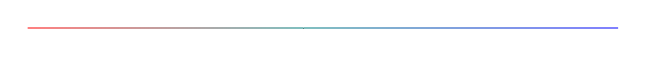
\begin{tikzpicture}
	\fill [left color=red!50, right color=teal!50] (0,0) rectangle (3.5,.01);
	\fill [left color=teal!50, right color=blue!50] (3.5,0) rectangle (7.5,.01);
	\end{tikzpicture}
\vspace{0.5cm}


%%%%%%%%%%%%%%%%%%%%%%%%%%%%%%%%%%%. \begin{ ------>. 
detsacado;  cuadro-naranja;  cuadro-gris;  miejercicio (solución extensa);  mipropuesto (solución corta y fuera del cuadro)

%%%%%%%%%%%%%%%%%%%%%%%%%%%%%%%%%%%. CURIOSIDAD
\vspace{1cm}
\color{ForestGreen!80}
\rule{250pt}{0.2pt}
Texto
\vspace{-8mm}
\begin{flushright}
\rule{250pt}{0.2pt}		
\end{flushright}	
\color{black}
\end{comment}
